%%%%%%%%%%%%%%%%%%%%%%%%%%%%%%%%%%%%%%%%%%%%%%%%%%%%%%%%%%%%%%%%%%%%%%%%%%%

\documentclass{standalone}

\usepackage{mathptmx}
\usepackage{tikz}
\usetikzlibrary{angles}
\usetikzlibrary{external}
\usetikzlibrary{quotes}
\tikzexternalize{unit-circle-30-degree}

%% We default to Times.
\renewcommand{\rmdefault}{ptm}
\renewcommand{\ttdefault}{pcr}
%% Enable Times/Palatino main text font.
\normalfont\selectfont

\newcommand{\comma}{,\,}
\newcommand{\tuple}[2]{\left({#1}\comma {#2}\right)}

%% The Cartesian coordinate system.
\newcommand{\cartesianCoordinate}{%%
  %% The x-axis.
  \draw[axisStyle] (xstart) -- (xend);
  \node at (xend) [right] {$x$};
  %% The y-axis.
  \draw[axisStyle] (ystart) -- (yend);
  \node at (yend) [above] {$y$};
}

%% A point that makes an angle of 30 degrees with respect to the
%% positive half of the x-axis.
\newcommand{\givenPoint}{%%
  \xyPoint{\xa}{\yb}{\tuple{\frac{\sqrt{3}}{2}}{\frac{1}{2}}}{above right}
  \radiusLine
}

%% The radius.
\newcommand{\radiusLine}{%%
  %% A line as the radius
  \draw[dashStyle] (origin) -- (point);
  %% Label the angle.
  \path pic["$\frac{\pi}{6}$",draw,->,thick,angle radius=1.5cm] {angle=xyRadius--origin--point};
}

%% The unit circle centred at the origin.
\newcommand{\unitCircle}{%%
  \draw[lineStyle] (origin) circle [radius=\radius];
}

%% A point on the Cartesian plane.
%%
%% #1 -- The x-coordinate of the point.
%% #2 -- The y-coordinate of the point.
%% #3 -- Label the point with this name.
%% #4 -- Where to place the label relative to the point.
\newcommand{\xyPoint}[4]{%%
  \node[nodeStyle] at (#1,#2) {};
  \node at (#1,#2) [#4] {$#3$};
}

%%%%%%%%%%%%%%%%%%%%%%%%%%%%%%%%%%%%%%%%%%%%%%%%%%%%%%%%%%%%%%%%%%%%%%%%%%%
%% A point that makes an angle of 30 degrees.
%%%%%%%%%%%%%%%%%%%%%%%%%%%%%%%%%%%%%%%%%%%%%%%%%%%%%%%%%%%%%%%%%%%%%%%%%%%

\begin{document}

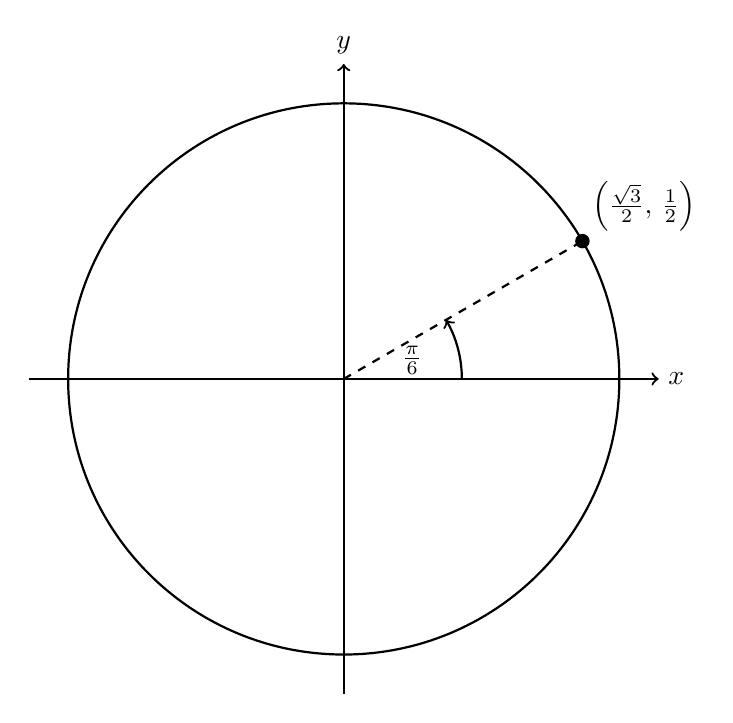
\begin{tikzpicture}[%%
  axisStyle/.style={->,thick},%%
  dashStyle/.style={-,thick,dashed},%%
  lineStyle/.style={-,thick},%%
  nodeStyle/.style={draw,inner sep=1.7pt,circle,fill=black,black}%%
]
%%
%%
\pgfmathsetmacro{\radius}{3.5}
\pgfmathsetmacro{\xa}{3.03108891324554}
\pgfmathsetmacro{\xhigh}{4}
\pgfmathsetmacro{\xlow}{-4}
\pgfmathsetmacro{\yb}{1.75}
\pgfmathsetmacro{\yhigh}{\xhigh}
\pgfmathsetmacro{\ylow}{\xlow}
%% The Cartesian coordinate system.
\coordinate (origin) at (0,0);
\coordinate (xend) at (\xhigh,0);
\coordinate (xstart) at (\xlow,0);
\coordinate (yend) at (0,\yhigh);
\coordinate (ystart) at (0,\ylow);
%% The generic angle.
\coordinate (point) at (\xa,\yb);
\coordinate (xyRadius) at (\radius,0);
%%
%%
%% Illustrate the unit circle.
\cartesianCoordinate
\unitCircle
\givenPoint
\end{tikzpicture}

\end{document}
